\documentclass {article}
\usepackage {pgfplots}
\pgfplotsset {compat=newest}

\pagestyle {empty}

\title {CS330 - Maximum Increasing Subarray Empirical Analysis}
\author {Andrew Knopf}
\date {June 18, 2026}

\begin{document}

\maketitle
This paper will explore the average values of the maximum subarray problem, utilizing Kadane's algorithm at several experiment sizes.


\section {Problem statement}
\indent\par The $maximum$ $subarray$ $problem$ is an algorithm that at a high level, takes an array and find the subarray that has the highest value. For example, if there was an array that had values: -2, 1, -3, 4, -1, 2, 1, -5, 4, then the maximum subarray would be: 4, -1, 2, 1, with a cumulative value of 6. The formula uses Kadane's algorithm, a brute force algorithm, which can be described as follows:

The question this paper will strive to answer is: given several sizes of subarrays, what is the relationship between 
https://www.calculator.net/average-calculator.html
\section {Experiment setup}
\indent \par The algorithm was run at a high level by creating an array of size N and initializing it's values to [$-n/3$, $2n/3$], then randomly shuffle it. The algorithm had several tests where the algorithm is run with a parent array of incrementing size, by 100, 200, 300 ... 1000, 2000, 3000... all the way up to 10,000. At each array size, the algorithm is run 200 times to create a more accurate output, and the results are printed to a text file. 
\par From there, the text I took the text file and calculated the averages of each data set by manually copying and pasting the programs .csv file output and into www.calculator.net/average-calculator to get the average value of the maximum subarray values.


% What is tikzpicture?
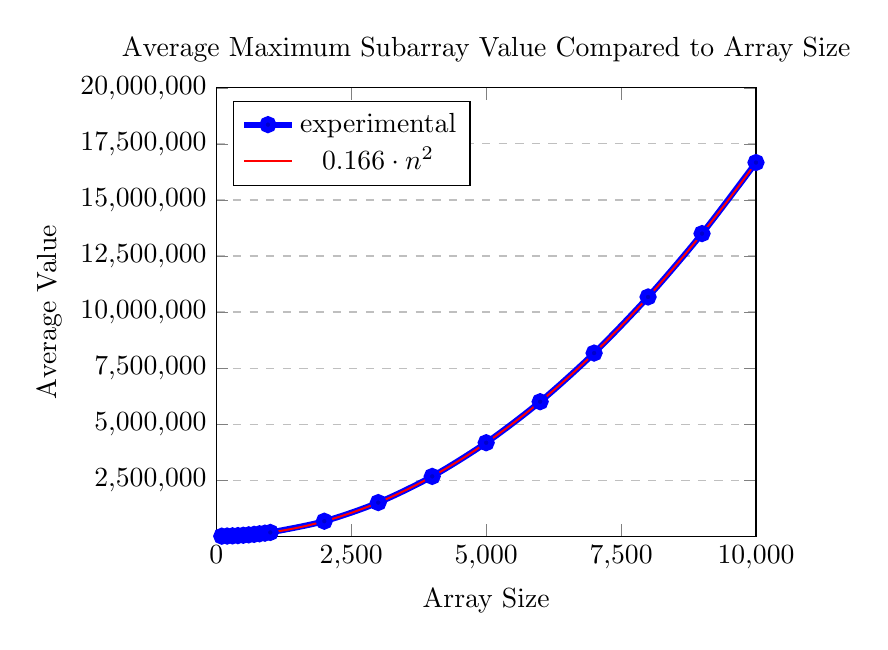
\begin{tikzpicture}

\begin{axis}
[
    legend style={at={(0.03,0.97)}, anchor=north west},
    title={Average Maximum Subarray Value Compared to Array Size},
    xlabel={Array Size},
    ylabel={Average Value},
    xmin=0, xmax=10000,
    ymin=0, ymax=20000000,
    scaled ticks = false,
    tick label style={/pgf/number format/fixed},
    xtick={0,2500,5000, 7500, 10000},
    ytick={2500000, 5000000, 7500000, 10000000, 12500000, 15000000, 17500000, 20000000},
    ymajorgrids=true,
    grid style=dashed
]

% Plot the data I analyzed

\addplot+ [color=blue, mark=*, smooth, line width = .75mm]
coordinates 
{
    (100, 1696.375 )
    (200  ,6782.135 )
    (300 , 14987.78 )
    (400 , 26777.905 )
    (500 , 41969.875 )
    (600  , 59952.465)
    (700 , 81882.495 )
    (800 , 107173.505)
    (900 , 134947.54 )
    (1000  , 166992.47)
    (2000  , 667921.10)
    (3000 , 1499784.5 )
    (4000 , 2667769.76 )
    (5000 , 4169857.04 )
    (6000  , 5999833.405 )
    (7000 , 8169058.015 )
    (8000 , 10671881.96 )
    (9000 , 13499686.83 )
    (10000  , 16669423.83)
};
\addlegendentryexpanded{experimental}
\addlegendentryexpanded{$0.166 \cdot n^2$}
\addplot+[line width=0.25mm,smooth,mark=,domain=0:10000] {(1/6) * x^2};
\end{axis}
\end{tikzpicture}

\section{Analysis}
\indent \par With the data shown above, it can be clearly seen that the maximum value of the subarray can be modeled accurately close to the line $0.166 \cdot n^2$. At larger and larger values the coefficient of $0.166$ becomes more and more insignificant (in a similar vein to Big-O notation). This leaves the relationship between the average maximum value of the subarray in regards to array size can be modeled with the line $n^2$. 
\indent \par Possible explanations for why the average maximum value can be modeled to this line are not easily explained. Because each experiment was run 200 times, it's unlikely that it was random chance. The most likely explanation is that because the values in the array itself are initialized to a range of [$-n/3$, $2n/3$], so there is a much higher possibility of positive values to initialize the array, this ensures a positive relationship. The magnitude of the relationship is due to the fact that as the array size grows, the larger the values can possibly be.
\indent \par The only major possible source of error could be in the process of copying and pasting the .csv values in the average calculator website. It's unlikely that the calculator produces incorrect results when used correctly, rather it's more likely that there was user error in the process of transferring several points of data manually. 

% Put a section in with no header
\section*{} 
DigiPen Institute of Technology (C) 2026
\end{document}